\documentclass{article}
\usepackage[utf8]{inputenc}
\usepackage{tikz}
\usepackage{amsmath, amssymb}
\usetikzlibrary{positioning}
\usetikzlibrary{fit}
\usepackage{color}

\begin{document}

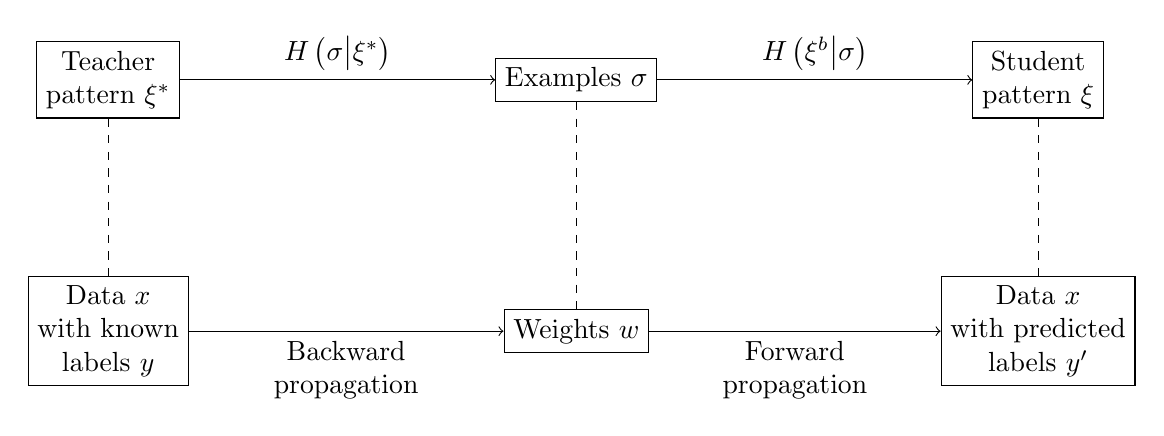
\begin{tikzpicture}[align = center, node distance = 2cm and 4cm]

\node[draw](xi^*){Teacher \\ pattern $\xi^*$};

\node[draw](sigma)[right = of xi^*]{Examples $\sigma$};

\node[draw](xi^b)[right = of sigma]{Student \\ pattern $\xi$};

\node[draw](v)[below = of xi^*]{Data $x$ \\ with known \\ labels $y$};

\node[draw](xi) at (sigma |- v){Weights $w$};

\node[draw](c)[below = of xi^b]{Data $x$ \\
with predicted \\ labels $y'$};

\draw[draw, ->](xi^*.east)--(sigma.west) node[midway, above]{$H \left( \sigma \big| \xi^* \right)$};

\draw[draw, ->](sigma.east)--(xi^b.west) node[midway, above]{$H \left( \xi^b \big| \sigma \right)$};

\draw[draw, ->](v.east)--(xi.west) node[midway, below]{Backward \\ propagation};

\draw[draw, ->](xi.east)--(c.west) node[midway, below]{Forward \\ propagation};

\draw[draw, dashed](xi^*.south)--(v.north);

\draw[draw, dashed](sigma.south)--(xi.north);

\draw[draw, dashed](xi^b.south)--(c.north);

\end{tikzpicture}

\end{document}